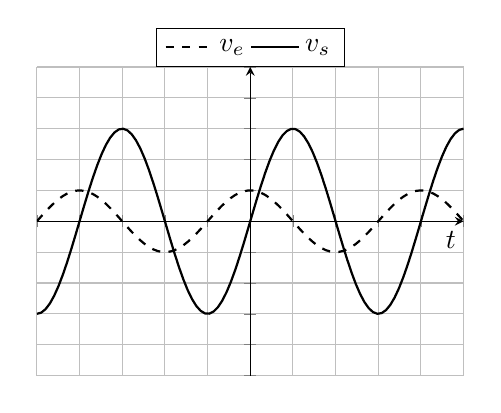
\begin{tikzpicture}
\begin{axis}[
    xlabel = \(t\),
    ylabel = {} ,
    domain = -5:5,
    ymin = -5,
    ymax = 5,
    samples = 100,
    axis x line = center,
    axis y line = center,
    xtick = {-5, -4, ..., 5},
    ytick = {-5, -4, ..., 5},
    xticklabels = {},
    yticklabels = {},
    grid = both,
    width = 7cm,
    height = 5.5cm,
    legend columns=2, 
    legend style={at={(0.5,1.0)}, anchor=south},
	x label style = {at={(0.97, .5)},anchor = north}
    ]
    \addplot [thick, dashed] {cos(2*x*180/4)};
    \addlegendentry{\(v_e\)}
    \addplot [thick] {3*cos(2*x*180/4-90)};
    \addlegendentry{\(v_s\)}
  \end{axis}
\end{tikzpicture}